\documentclass[aspectratio=169,10pt]{beamer}

\usepackage[T1]{fontenc}
\usepackage[scaled=0.94]{helvet}
\usepackage{courier}
\usepackage{amsmath}
\usepackage{booktabs}
\usepackage{array}
\usepackage{tikz}
\usepackage{xcolor}
\usepackage{ragged2e}
\usetikzlibrary{arrows.meta,positioning,shapes.geometric,calc,fit}

\renewcommand{\familydefault}{\sfdefault}

\definecolor{Navy}{HTML}{17324D}
\definecolor{Blue}{HTML}{2878B5}
\definecolor{Cyan}{HTML}{39A9B8}
\definecolor{Mint}{HTML}{DDF4F1}
\definecolor{Amber}{HTML}{F2A93B}
\definecolor{Red}{HTML}{D95D59}
\definecolor{Green}{HTML}{37966F}
\definecolor{Ink}{HTML}{243642}
\definecolor{Slate}{HTML}{60717B}
\definecolor{Pale}{HTML}{F4F7F9}
\definecolor{Line}{HTML}{D7E0E5}

\setbeamercolor{normal text}{fg=Ink,bg=white}
\setbeamercolor{structure}{fg=Blue}
\setbeamercolor{frametitle}{fg=Navy,bg=white}
\setbeamercolor{title}{fg=white}
\setbeamercolor{subtitle}{fg=Mint}
\setbeamercolor{block title}{fg=white,bg=Navy}
\setbeamercolor{block body}{fg=Ink,bg=Pale}
\setbeamercolor{alerted text}{fg=Red}
\setbeamertemplate{navigation symbols}{}
\setbeamertemplate{itemize item}{\color{Blue}\small$\blacktriangleright$}
\setbeamertemplate{itemize subitem}{\color{Cyan}\scriptsize$\bullet$}
\setbeamertemplate{enumerate item}{\color{Blue}\insertenumlabel.}
\setbeamertemplate{frametitle}{
  \vspace{0.35cm}
  \hspace{0.25cm}\insertframetitle
  \par\vspace{0.12cm}
  \hspace{0.25cm}\color{Line}\rule{13.85cm}{0.5pt}
}
\setbeamertemplate{footline}{
  \leavevmode
  \vspace{0.08cm}
  \hbox to 0.995\paperwidth{
    \hspace{0.45cm}
    \scriptsize\color{Slate}Global Congestion-Balanced Slotting Proposal
    \hfill
    \scriptsize\color{Slate}\insertframenumber/\inserttotalframenumber
    \hspace{0.45cm}
  }
  \vspace{0.10cm}
}

\newcommand{\key}[1]{\textcolor{Blue}{\textbf{#1}}}
\newcommand{\metric}[1]{\textcolor{Navy}{\textbf{\Large #1}}}
\newcommand{\smallcaps}[1]{\textcolor{Slate}{\scriptsize\MakeUppercase{#1}}}
\newcommand{\pill}[2]{%
  \tikz[baseline=(X.base)]\node[
    rounded corners=2pt,fill=#1!12,text=#1,
    inner xsep=6pt,inner ysep=3pt,font=\scriptsize\bfseries
  ](X){#2};%
}

\tikzset{
  flow/.style={
    rounded corners=4pt,draw=Line,very thick,fill=white,
    minimum height=1.05cm,text width=2.35cm,align=center,
    font=\small\bfseries,text=Ink
  },
  decision/.style={
    diamond,aspect=2.1,draw=Amber,very thick,fill=Amber!10,
    text width=2.2cm,align=center,font=\scriptsize\bfseries,text=Ink
  },
  arrow/.style={-{Stealth[length=2.7mm]},very thick,draw=Slate},
  card/.style={
    rounded corners=5pt,draw=Line,fill=Pale,
    inner sep=8pt,align=left,text=Ink
  }
}

\title{Global Congestion-Balanced\\Slotting Optimization}
\subtitle{Exact layout assignment for smoother warehouse traffic and lower downtime}
\author{Layout Management System Proposal}
\date{27 July 2026}

\begin{document}

\begin{frame}[plain]
  \begin{tikzpicture}[remember picture,overlay]
    \fill[Navy] (current page.south west) rectangle (current page.north east);
    \fill[Blue] ($(current page.south west)+(0,0)$)
      rectangle ($(current page.south west)+(0.28,9)$);
    \fill[Cyan] ($(current page.south west)+(0.28,0)$)
      rectangle ($(current page.south west)+(0.38,9)$);
    \node[anchor=north west,text width=12.8cm] at
      ($(current page.north west)+(1.25,-1.35)$) {
        {\color{white}\fontsize{25}{29}\selectfont\bfseries
          Global Congestion-Balanced\\Slotting Optimization}
      };
    \node[anchor=north west,text width=11.5cm] at
      ($(current page.north west)+(1.28,-3.65)$) {
        {\color{Mint}\Large
          Exact layout assignment for smoother warehouse traffic\\
          and lower operational downtime}
      };
    \node[anchor=south west] at
      ($(current page.south west)+(1.28,1.05)$) {
        {\color{white}\small Layout Management System Proposal}
      };
    \node[anchor=south east] at
      ($(current page.south east)+(-1.0,1.05)$) {
        {\color{Mint}\small 27 July 2026}
      };
    \draw[Cyan,very thick]
      ($(current page.north west)+(1.28,-5.35)$) --
      ($(current page.north west)+(8.8,-5.35)$);
  \end{tikzpicture}
\end{frame}

\begin{frame}{Decision requested}
  \small
  \begin{columns}[T,onlytextwidth]
    \column{0.58\textwidth}
      {\large\bfseries Approve exact congestion-balanced placement}

      \vspace{0.18cm}
      Assign complete movable units across the whole warehouse rather than
      relying only on pair swaps.

      \vspace{0.18cm}
      \begin{itemize}
        \item Globally minimize the worst movement bottleneck
        \item Prevent popular racks from clustering in one zone or aisle
        \item Preserve every existing storage hard rule
        \item Constrain additional travel and report the optimality gap
      \end{itemize}

    \column{0.38\textwidth}
      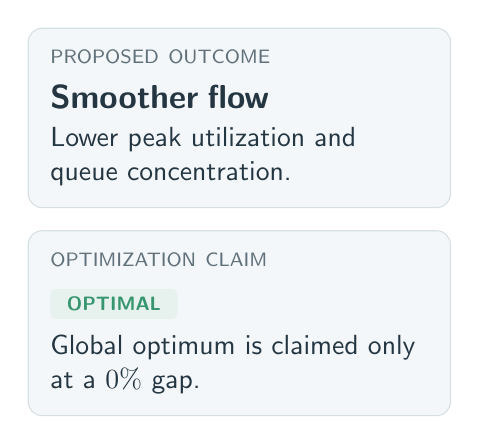
\begin{tikzpicture}
        \node[card,text width=4.8cm] (outcome) {
          \smallcaps{Proposed outcome}\\[4pt]
          \textbf{\large Smoother flow}\\[2pt]
          Lower peak utilization and queue concentration.
        };
        \node[card,text width=4.8cm,below=0.28cm of outcome] {
          \smallcaps{Optimization claim}\\[4pt]
          \pill{Green}{OPTIMAL}\\[4pt]
          Global optimum is claimed only at a \(0\%\) gap.
        };
      \end{tikzpicture}
  \end{columns}
\end{frame}

\begin{frame}{Problem to solve}
  \small
  \begin{columns}[T,onlytextwidth]
    \column{0.47\textwidth}
      \begin{block}{Current operational risk}
        Popular shelves or totes can accumulate in the same zone, aisle,
        lift, or crane service area.
      \end{block}
      \vspace{0.18cm}
      This concentrates traffic even when total warehouse capacity is adequate.

      \vspace{0.25cm}
      \begin{itemize}
        \item Queueing at shared entrances and transfer points
        \item Uneven robot or crane workload
        \item Longer waiting time and lower throughput
      \end{itemize}

    \column{0.49\textwidth}
      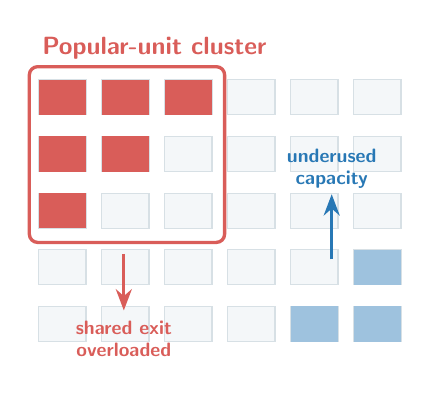
\begin{tikzpicture}[x=0.8cm,y=0.72cm]
        \foreach \x in {0,...,5}
          \foreach \y in {0,...,4}
            \draw[Line,fill=Pale] (\x,\y) rectangle ++(0.75,0.62);
        \foreach \p in {(0,4),(1,4),(0,3),(1,3),(2,4),(0,2)}
          \fill[Red] \p rectangle ++(0.75,0.62);
        \foreach \p in {(4,0),(5,0),(5,1)}
          \fill[Blue!45] \p rectangle ++(0.75,0.62);
        \draw[Red,very thick,rounded corners=3pt] (-0.15,1.75)
          rectangle (2.95,4.85);
        \node[Red,font=\small\bfseries,anchor=west] at (-0.1,5.18)
          {Popular-unit cluster};
        \draw[arrow,Red] (1.35,1.55) -- (1.35,0.55);
        \node[font=\scriptsize\bfseries,text=Red,align=center] at (1.35,0.05)
          {shared exit\\overloaded};
        \draw[arrow,Blue] (4.65,1.45) -- (4.65,2.6);
        \node[font=\scriptsize\bfseries,text=Blue,align=center] at (4.65,3.05)
          {underused\\capacity};
      \end{tikzpicture}
  \end{columns}
\end{frame}

\begin{frame}{Success definition}
  \begin{columns}[T,onlytextwidth]
    \column{0.24\textwidth}
      \smallcaps{Primary}
      \vspace{0.12cm}

      \metric{Peak}

      Minimize the maximum normalized load across lanes, lifts, cranes,
      intersections, and transfer points.

    \column{0.24\textwidth}
      \smallcaps{Spatial balance}
      \vspace{0.12cm}

      \metric{Local}

      Prevent high-visit movable units from accumulating in one compatible
      zone or shared-resource neighbourhood.

    \column{0.24\textwidth}
      \smallcaps{Service quality}
      \vspace{0.12cm}

      \metric{P95}

      Reduce the high-load tail so traffic is smooth across more than a single
      worst bottleneck.

    \column{0.24\textwidth}
      \smallcaps{Guardrail}
      \vspace{0.12cm}

      \metric{Travel}

      Keep total expected travel within a configured increase from the
      starting layout.
  \end{columns}

  \vspace{0.5cm}
  \begin{center}
    \pill{Blue}{BALANCE BY CAPACITY, NOT RAW VISITS}
    \hspace{0.3cm}
    \pill{Green}{ALL HARD RULES REMAIN ENFORCED}
  \end{center}
\end{frame}

\begin{frame}{Current method versus proposed method}
  \begin{columns}[T,onlytextwidth]
    \column{0.47\textwidth}
      \begin{block}{Current: greedy pair swaps}
        \begin{itemize}
          \item Starts from an existing, ABC, or affinity layout
          \item Exchanges two complete handling units
          \item Accepts immediate lexicographic improvements
          \item Stops after a limited number of iterations
        \end{itemize}
      \end{block}
      \vspace{0.2cm}
      \pill{Amber}{FAST}\quad
      \pill{Red}{LOCAL OPTIMUM RISK}

    \column{0.47\textwidth}
      \begin{block}{Proposed: exact global assignment}
        \begin{itemize}
          \item Assigns every movable unit to a compatible location
          \item Evaluates resource, zone, and local concentration together
          \item Uses branch-and-bound to prove the best model solution
          \item Reports incumbent, lower bound, and optimality gap
        \end{itemize}
      \end{block}
      \vspace{0.2cm}
      \pill{Green}{GLOBALLY AUDITABLE}\quad
      \pill{Blue}{TIME-BOUNDED OPTION}
  \end{columns}
\end{frame}

\begin{frame}{Universal movable-unit abstraction}
  \begin{center}
    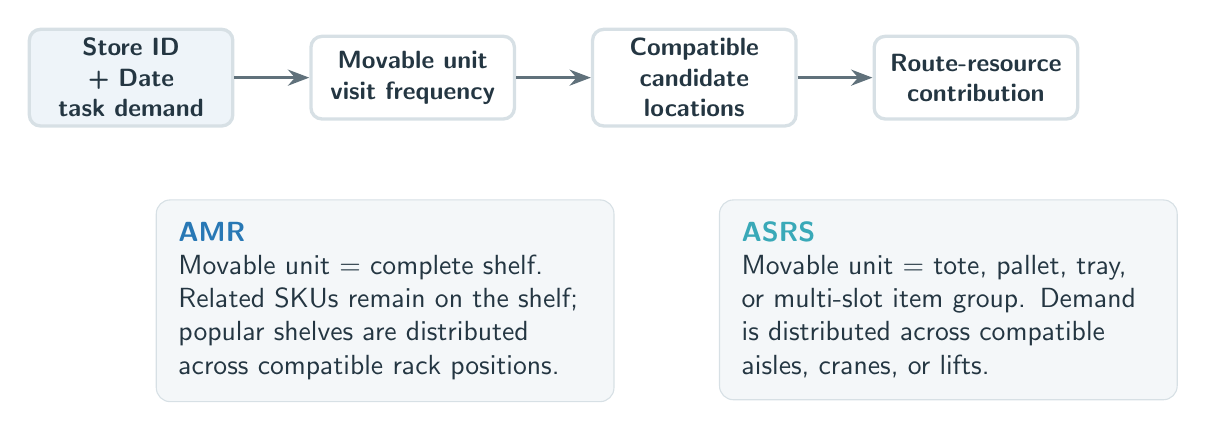
\begin{tikzpicture}[node distance=0.75cm and 0.95cm]
      \node[flow,fill=Blue!8] (demand) {Store ID + Date\\task demand};
      \node[flow,right=of demand] (unit) {Movable unit\\visit frequency};
      \node[flow,right=of unit] (location) {Compatible\\candidate locations};
      \node[flow,right=of location] (resource) {Route-resource\\contribution};
      \draw[arrow] (demand) -- (unit);
      \draw[arrow] (unit) -- (location);
      \draw[arrow] (location) -- (resource);

      \node[card,text width=5.25cm,below=1.0cm of unit,xshift=-0.35cm] (amr) {
        \textbf{\textcolor{Blue}{AMR}}\\
        Movable unit = complete shelf. Related SKUs remain on the shelf;
        popular shelves are distributed across compatible rack positions.
      };
      \node[card,text width=5.25cm,below=1.0cm of resource,xshift=-0.35cm] (asrs) {
        \textbf{\textcolor{Cyan}{ASRS}}\\
        Movable unit = tote, pallet, tray, or multi-slot item group.
        Demand is distributed across compatible aisles, cranes, or lifts.
      };
    \end{tikzpicture}
  \end{center}

  \vspace{0.15cm}
  \begin{center}
    One optimization interface; system-specific units and resource networks.
  \end{center}
\end{frame}

\begin{frame}{Demand and traffic model}
  \begin{columns}[T,onlytextwidth]
    \column{0.48\textwidth}
      \smallcaps{Historical demand}
      \[
        v_u = \sum_{t \in \mathcal{T}}
        \mathbf{1}\{\text{task }t\text{ requires unit }u\}
      \]
      \begin{itemize}
        \item One task is one \(\text{Store ID}+\text{Date}\)
        \item AMR shelf is counted once per task
        \item ASRS counts each required physical retrieval
      \end{itemize}

    \column{0.48\textwidth}
      \smallcaps{Precomputed route contribution}
      \[
        a_{ulr} =
        v_u \times
        \mathbf{1}\{\text{route from }l\text{ uses }r\}
      \]
      \begin{itemize}
        \item \(u\): movable unit
        \item \(l\): candidate storage location
        \item \(r\): shared movement resource
      \end{itemize}
  \end{columns}

  \vspace{0.35cm}
  \begin{block}{Fixed-route scope}
    Shortest routes are precomputed for every candidate location. This makes
    layout assignment exact and tractable while matching the current expected-flow model.
  \end{block}
\end{frame}

\begin{frame}{Exact placement model}
  \begin{columns}[T,onlytextwidth]
    \column{0.48\textwidth}
      \smallcaps{Decision variable}
      \[
        x_{ul} =
        \begin{cases}
          1 & \text{unit \(u\) is assigned to location \(l\)}\\
          0 & \text{otherwise}
        \end{cases}
      \]

      \smallcaps{One location per unit}
      \[
        \sum_{l \in L(u)} x_{ul}=1
        \qquad \forall u
      \]

    \column{0.48\textwidth}
      \smallcaps{Location occupancy}
      \[
        \sum_{u:\,l\in L(u)} x_{ul}\leq 1
        \qquad \forall l
      \]

      \smallcaps{Resource utilization}
      \[
        q_r=\frac{1}{C_r}
        \sum_u \sum_{l\in L(u)} a_{ulr}x_{ul}
      \]
  \end{columns}

  \vspace{0.3cm}
  \begin{center}
    \(L(u)\) contains only hard-rule-compatible locations;
    invalid placement variables are never created.
  \end{center}
\end{frame}

\begin{frame}{Congestion must be measured at three levels}
  \begin{columns}[T,onlytextwidth]
    \column{0.31\textwidth}
      \begin{block}{1. Shared resource}
        Lane, aisle entrance, lift, crane, intersection, conveyor, or transfer point.
        \[
          Q^{R}=\max_r q_r
        \]
      \end{block}

    \column{0.31\textwidth}
      \begin{block}{2. Zone}
        Workload normalized by the compatible zone's service capacity.
        \[
          Q^{Z}=\max_z
          \frac{\sum_{u,l\in z}v_ux_{ul}}{C_z}
        \]
      \end{block}

    \column{0.31\textwidth}
      \begin{block}{3. Local neighbourhood}
        Racks sharing a physical entrance, lift, crane, or defined grid window.
        \[
          Q^{N}=\max_n
          \frac{\sum_{u,l\in n}v_ux_{ul}}{C_n}
        \]
      \end{block}
  \end{columns}

  \vspace{0.35cm}
  \begin{center}
    \pill{Blue}{RECOMMENDATION}
    Define neighbourhoods from shared physical resources before using arbitrary grid windows.
  \end{center}
\end{frame}

\begin{frame}{Lexicographic global objective}
  \begin{center}
    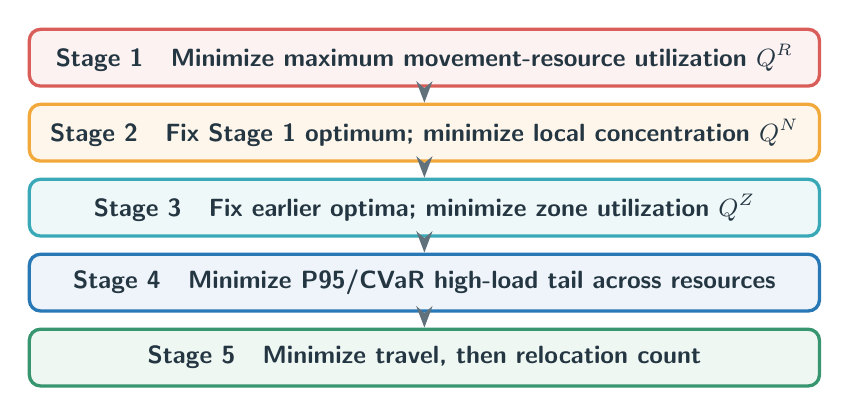
\begin{tikzpicture}[node distance=0.19cm]
      \node[flow,minimum height=0.72cm,text width=9.8cm,fill=Red!8,draw=Red] (one) {
        \textbf{Stage 1}\quad Minimize maximum movement-resource utilization \(Q^R\)
      };
      \node[flow,minimum height=0.72cm,text width=9.8cm,below=of one,fill=Amber!10,draw=Amber] (two) {
        \textbf{Stage 2}\quad Fix Stage 1 optimum; minimize local concentration \(Q^N\)
      };
      \node[flow,minimum height=0.72cm,text width=9.8cm,below=of two,fill=Cyan!8,draw=Cyan] (three) {
        \textbf{Stage 3}\quad Fix earlier optima; minimize zone utilization \(Q^Z\)
      };
      \node[flow,minimum height=0.72cm,text width=9.8cm,below=of three,fill=Blue!8,draw=Blue] (four) {
        \textbf{Stage 4}\quad Minimize P95/CVaR high-load tail across resources
      };
      \node[flow,minimum height=0.72cm,text width=9.8cm,below=of four,fill=Green!8,draw=Green] (five) {
        \textbf{Stage 5}\quad Minimize travel, then relocation count
      };
      \draw[arrow] (one) -- (two);
      \draw[arrow] (two) -- (three);
      \draw[arrow] (three) -- (four);
      \draw[arrow] (four) -- (five);
    \end{tikzpicture}
  \end{center}

  \vspace{0.05cm}
  Earlier objectives cannot be sacrificed for a later convenience metric.
\end{frame}

\begin{frame}{Queue-risk penalty for smoother traffic}
  \begin{columns}[T,onlytextwidth]
    \column{0.52\textwidth}
      Average load is not enough: waiting time rises sharply as utilization approaches capacity.

      \vspace{0.25cm}
      Use a convex piecewise-linear penalty:

      \begin{center}
        \begin{tabular}{@{}ll@{}}
          \toprule
          Utilization & Marginal penalty\\
          \midrule
          \(0\)--\(60\%\) & Low\\
          \(60\)--\(75\%\) & Moderate\\
          \(75\)--\(90\%\) & High\\
          \(>90\%\) & Extreme\\
          \bottomrule
        \end{tabular}
      \end{center}

    \column{0.43\textwidth}
      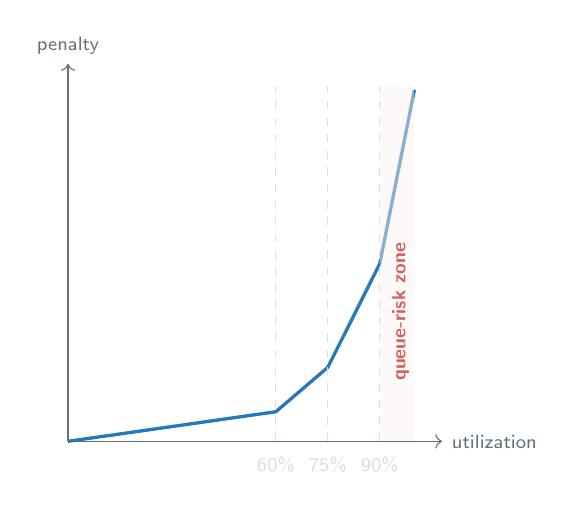
\begin{tikzpicture}[x=4.4cm,y=0.047cm]
        \draw[->,Slate] (0,0) -- (1.08,0) node[right,font=\scriptsize]{utilization};
        \draw[->,Slate] (0,0) -- (0,102) node[above,font=\scriptsize]{penalty};
        \draw[very thick,Blue] (0,0) -- (.60,8) -- (.75,20)
          -- (.90,48) -- (1.0,95);
        \foreach \x/\t in {.60/60\%,.75/75\%,.90/90\%}
          \draw[Line,dashed] (\x,0) -- (\x,96)
            node[below=2pt,at start,font=\scriptsize]{\t};
        \fill[Red!8,opacity=.45] (.90,0) rectangle (1.0,96);
        \node[Red,font=\scriptsize\bfseries,rotate=90] at (.96,35)
          {queue-risk zone};
      \end{tikzpicture}
  \end{columns}

  \vspace{-0.15cm}
  \begin{center}
    \small\textbf{\textcolor{Blue}{Effect:}} spread traffic before a bottleneck
    reaches unstable utilization.
  \end{center}
\end{frame}

\begin{frame}{Hard rules remain non-negotiable}
  \begin{columns}[T,onlytextwidth]
    \column{0.48\textwidth}
      \begin{itemize}
        \item Chilled inventory remains in chilled-compatible storage
        \item Ambient standard and oversize segments remain non-mixed
        \item Dimensions, rotation, weight, and contiguous footprint must fit
        \item Known overweight inventory remains on its required ergonomic level
        \item Custom inherited zone/rack/slot attributes remain enforced
      \end{itemize}

    \column{0.48\textwidth}
      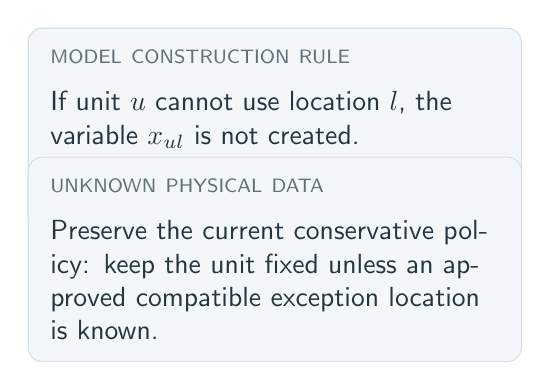
\begin{tikzpicture}
        \node[card,text width=5.7cm] {
          \smallcaps{Model construction rule}\\[5pt]
          If unit \(u\) cannot use location \(l\), the variable \(x_{ul}\)
          is not created.\\[8pt]
          \pill{Green}{INVALID PLACEMENT IMPOSSIBLE}
        };
        \node[card,text width=5.7cm,below=0.35cm] {
          \smallcaps{Unknown physical data}\\[5pt]
          Preserve the current conservative policy: keep the unit fixed
          unless an approved compatible exception location is known.
        };
      \end{tikzpicture}
  \end{columns}
\end{frame}

\begin{frame}{End-to-end solver workflow}
  \begin{center}
    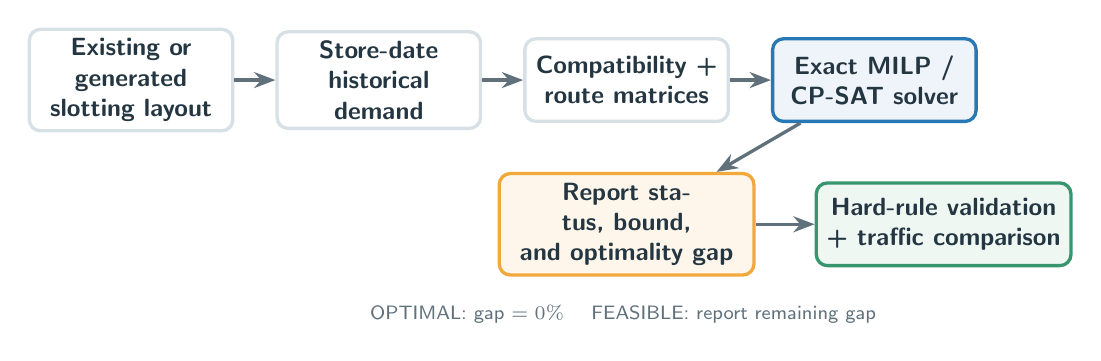
\begin{tikzpicture}[node distance=0.45cm and 0.52cm]
      \node[flow] (layout) {Existing or generated\\slotting layout};
      \node[flow,right=of layout] (history) {Store-date\\historical demand};
      \node[flow,right=of history] (matrix) {Compatibility +\\route matrices};
      \node[flow,right=of matrix,fill=Blue!8,draw=Blue] (solver) {Exact MILP /\\CP-SAT solver};
      \draw[arrow] (layout) -- (history);
      \draw[arrow] (history) -- (matrix);
      \draw[arrow] (matrix) -- (solver);

      \node[flow,text width=3.0cm,below=0.62cm of matrix,fill=Amber!10,draw=Amber] (status) {
        Report status, bound,\\and optimality gap
      };
      \draw[arrow] (solver) -- (status);
      \node[flow,right=0.75cm of status,text width=3.0cm,fill=Green!8,draw=Green] (validate) {
        Hard-rule validation\\+ traffic comparison
      };
      \draw[arrow] (status) -- (validate);
      \node[anchor=north,font=\scriptsize,text=Slate,align=center]
        at ($(status.south)+(0,-0.24)$) {
          OPTIMAL: gap \(=0\%\) \quad FEASIBLE: report remaining gap
        };
    \end{tikzpicture}
  \end{center}
\end{frame}

\begin{frame}{Integration with the current application}
  \begin{columns}[T,onlytextwidth]
    \column{0.49\textwidth}
      \begin{block}{Keep both baseline workflows}
        \begin{enumerate}
          \item Optimize an existing \texttt{.slotting.json}
          \item Generate ABC or ABC + affinity, then optimize
        \end{enumerate}
      \end{block}

      \vspace{0.15cm}
      Add a solver-mode selector:

      \vspace{0.12cm}
      \pill{Blue}{QUICK HEURISTIC}\quad
      \pill{Green}{EXACT / BOUNDED}

    \column{0.47\textwidth}
      \begin{block}{New exact-mode settings}
        \begin{itemize}
          \item Solve-time limit
          \item Maximum travel increase
          \item Optimality-gap target
          \item Neighbourhood definition
          \item Solver backend
        \end{itemize}
      \end{block}

      Save the model status, bound, gap, objectives, and placement audit in the
      resulting \texttt{.slotting.json}.
  \end{columns}
\end{frame}

\begin{frame}{Solver strategy and global-optimum claim}
  \begin{columns}[T,onlytextwidth]
    \column{0.47\textwidth}
      \begin{block}{Exact mode}
        Continue branch-and-bound until:
        \[
          \text{optimality gap}=0\%
        \]
        Output status: \pill{Green}{OPTIMAL}
      \end{block}

      Recommended backend:
      \begin{itemize}
        \item Gurobi or CPLEX for strongest MILP performance
        \item OR-Tools CP-SAT for an open-source pilot
      \end{itemize}

    \column{0.47\textwidth}
      \begin{block}{Time-bounded mode}
        Stop after a configured duration and report:
        \[
          \text{gap}=
          \frac{\text{incumbent}-\text{bound}}
               {|\text{incumbent}|}
        \]
        Output status: \pill{Amber}{FEASIBLE}
      \end{block}

      A feasible solution must never be labelled globally optimal.
  \end{columns}
\end{frame}

\begin{frame}{Validation: optimization first, simulation second}
  \begin{center}
    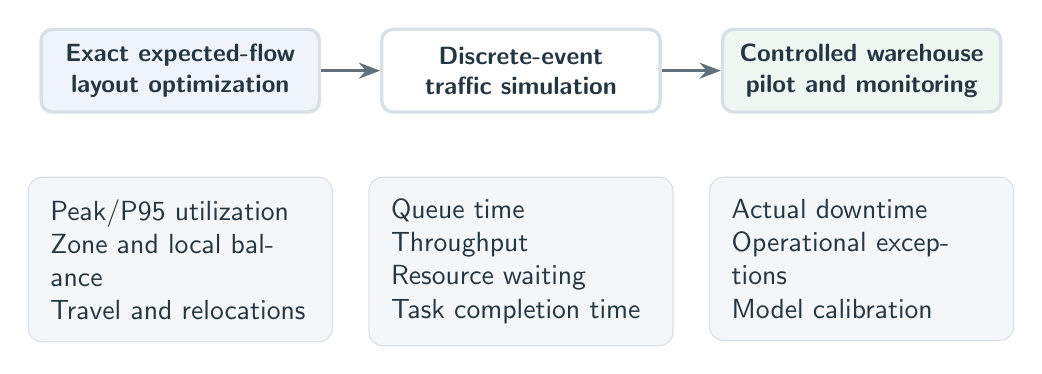
\begin{tikzpicture}[node distance=0.75cm]
      \node[flow,text width=3.3cm,fill=Blue!8] (exact) {
        Exact expected-flow\\layout optimization
      };
      \node[flow,text width=3.3cm,right=of exact] (sim) {
        Discrete-event\\traffic simulation
      };
      \node[flow,text width=3.3cm,right=of sim,fill=Green!8] (pilot) {
        Controlled warehouse\\pilot and monitoring
      };
      \draw[arrow] (exact) -- (sim);
      \draw[arrow] (sim) -- (pilot);

      \node[card,text width=3.3cm,below=0.8cm of exact] {
        Peak/P95 utilization\\Zone and local balance\\Travel and relocations
      };
      \node[card,text width=3.3cm,below=0.8cm of sim] {
        Queue time\\Throughput\\Resource waiting\\Task completion time
      };
      \node[card,text width=3.3cm,below=0.8cm of pilot] {
        Actual downtime\\Operational exceptions\\Model calibration
      };
    \end{tikzpicture}
  \end{center}

  \vspace{0.15cm}
  Exact optimization proves the best layout for the fixed-route model;
  simulation tests whether that model predicts real operational improvement.
\end{frame}

\begin{frame}{Delivery plan}
  \begin{center}
    \scriptsize
    \begin{tabular}{@{}p{2.1cm}p{5.8cm}p{1.65cm}p{1.9cm}@{}}
      \toprule
      \textbf{Phase} & \textbf{Deliverable} & \textbf{Estimate} & \textbf{Exit evidence}\\
      \midrule
      1. Data model &
      Movable-unit, candidate-location, resource, zone, and neighbourhood matrices &
      3--4 days & Matrix tests\\
      \addlinespace
      2. Exact solver &
      Placement constraints, lexicographic objectives, warm start, bounds, and gap &
      5--7 days & Small-instance proof\\
      \addlinespace
      3. Product integration &
      Solver mode, progress/cancel, JSON audit, map comparison, and error handling &
      3--4 days & GUI workflow test\\
      \addlinespace
      4. Validation &
      Benchmark layouts, simulation comparison, performance tuning, and documentation &
      4--6 days & Acceptance report\\
      \bottomrule
    \end{tabular}
  \end{center}

  \vspace{0.4cm}
  \begin{center}
    \pill{Blue}{TOTAL: 15--21 ENGINEERING DAYS}
    \hspace{0.25cm}
    \pill{Green}{PILOT: APPROXIMATELY 3--4 WEEKS}
  \end{center}
\end{frame}

\begin{frame}{Key risks and controls}
  \begin{columns}[T,onlytextwidth]
    \column{0.48\textwidth}
      \begin{block}{Solver runtime}
        \textbf{Risk:} assignment size grows with units \(\times\) locations.\\
        \textbf{Control:} compatibility pruning, warm starts, symmetry breaking,
        and explicit exact/time-bounded modes.
      \end{block}

      \begin{block}{Weak capacity data}
        \textbf{Risk:} relative loads may not represent real bottlenecks.\\
        \textbf{Control:} support measured capacities and preserve transparent
        relative-mode reporting.
      \end{block}

    \column{0.48\textwidth}
      \begin{block}{Static-route approximation}
        \textbf{Risk:} controllers may reroute around congestion.\\
        \textbf{Control:} validate with simulation and later add scenario or
        route-choice extensions.
      \end{block}

      \begin{block}{Operational churn}
        \textbf{Risk:} mathematically strong layouts may relocate too many units.\\
        \textbf{Control:} travel cap, relocation minimization, and operator-visible
        move audit.
      \end{block}
  \end{columns}
\end{frame}

\begin{frame}{Acceptance criteria}
  \begin{columns}[T,onlytextwidth]
    \column{0.49\textwidth}
      \smallcaps{Functional}
      \begin{itemize}
        \item Existing-layout and full-pipeline entry paths both work
        \item AMR and ASRS movable units use the same solver interface
        \item Every current hard rule is validated before and after solving
        \item Result JSON records status, bound, gap, objectives, and moves
      \end{itemize}

    \column{0.47\textwidth}
      \smallcaps{Performance and quality}
      \begin{itemize}
        \item Exact benchmark instances finish with \(0\%\) gap
        \item Time-bounded runs return a valid incumbent and honest gap
        \item Peak and local concentration do not worsen
        \item Travel remains inside the configured limit
      \end{itemize}
  \end{columns}

  \vspace{0.45cm}
  \begin{block}{Pilot success measure}
    Simulation or controlled operations show lower queue time and smoother
    resource utilization without violating storage compatibility or increasing
    travel beyond policy.
  \end{block}
\end{frame}

\begin{frame}[plain]
  \begin{tikzpicture}[remember picture,overlay]
    \fill[Navy] (current page.south west) rectangle (current page.north east);
    \node[anchor=north west,text width=12.5cm] at
      ($(current page.north west)+(1.25,-1.2)$) {
        {\color{white}\fontsize{24}{28}\selectfont\bfseries
          Recommended approval}
      };
    \node[anchor=north west,text width=12.8cm] at
      ($(current page.north west)+(1.28,-2.45)$) {
        {\color{Mint}\Large
          Proceed with a fixed-route exact pilot that minimizes resource,
          local, and zone congestion under all existing hard rules.}
      };
    \node[anchor=north west,text width=11.9cm] at
      ($(current page.north west)+(1.28,-4.25)$) {
        {\color{white}\large
          Deliver both exact and time-bounded modes. Validate predicted
          downtime reduction with discrete-event simulation before deployment.}
      };
    \node[anchor=south west] at
      ($(current page.south west)+(1.28,1.35)$) {
        \pill{Green}{GLOBAL WHEN GAP = 0\%}
        \hspace{0.25cm}
        \pill{Cyan}{AUDITABLE}
        \hspace{0.25cm}
        \pill{Amber}{OPERATIONALLY CONSTRAINED}
      };
  \end{tikzpicture}
\end{frame}

\end{document}
